\documentclass[11pt,a4paper]{article}
\usepackage[margin=2.5cm]{geometry}
\usepackage{amsmath,amssymb,graphicx,booktabs,siunitx,flafter,placeins}
\usepackage[tableposition=top]{caption}
\usepackage[hidelinks]{hyperref}
\sisetup{detect-all}
\setcounter{topnumber}{3}
\renewcommand{\topfraction}{0.8}
\newcommand{\R}{\mathbb{R}}
\newcommand{\1}{\mathbf{1}}
\title{Handwritten Digit Recognition: From Scratch to Curated Data}
\author{Immanuel Albrecht \and Claude Opus 5.5 (Anthropic)}
\date{October 2026}
\pdfinfoomitdate=1  % no creation/modification date in the PDF
\pdftrailerid{}
\begin{document}
\maketitle

% Structure (D26): main text (sections 1-7) at most 10 pages, details in the appendix.

\section{Overview}
\label{sec:overview}

This report documents a small but complete machine-learning project on MNIST, from the
mathematics to clean data: a neural network written by hand in NumPy and verified with a
gradient check, a regularised CNN in PyTorch with controlled experiments, an evaluation with
confidence intervals and calibration, and a curation loop in which suspicious training and test
labels are found with cross-validated confident learning, reviewed in a browser tool and used to
retrain the model. Everything runs on a laptop with an 8\,GB GPU. Every run is a folder with its
configuration, git commit, dataset version (a hash of the curation decisions), metrics and
per-sample predictions, so each number in this report can be reproduced from the repository.

\begin{table}[ht]
  \centering
  \small
  \caption{Main results on the original MNIST test set (10\,000 images). E7 and E8: mean
    $\pm$ standard deviation over three seeds.}
  \label{tab:summary}
  \begin{tabular}{llr}
    \toprule
    Model & Experiment & Test accuracy [\%] \\
    \midrule
    Logistic regression & E1 & 92.54 \\
    $k$-nearest neighbours ($k = 3$) & E1 & 96.90 \\
    MLP, own NumPy implementation, Adam, 20 epochs & E2 & 97.84 \\
    The same MLP in PyTorch & E3 & 97.90 \\
    Small CNN, 15 epochs & E4 & 98.95 \\
    Regularised CNN & E7 & $99.67 \pm 0.03$ \\
    Ensemble of the five cross-validation models & Sec.~\ref{sec:curation} & 99.73 \\
    Regularised CNN trained on the curated data & E8 & $99.60 \pm 0.09$ \\
    \bottomrule
  \end{tabular}
\end{table}

The appendix holds the side experiments, the optimiser derivations and the full tables.

\section{Backpropagation derivation}
\label{sec:backprop}

The network of plan step~7.2 is a multilayer perceptron $784 \to 256 \to 128 \to 10$ with ReLU
activations and a softmax output trained with cross-entropy; it has \num{235146} parameters.
Everything in this section is implemented by hand in NumPy (\texttt{digits.numpy\_net}); no
automatic differentiation is used.

\subsection{Forward pass}
For a single image $x \in \R^{784}$ (pixels scaled to $[0,1]$ and standardised with the
training-set mean $0.1307$ and standard deviation $0.3081$) and layers $l = 1, 2, 3$:
\begin{align}
  a^{(0)} &= x, &
  z^{(l)} &= W^{(l)} a^{(l-1)} + b^{(l)}, &
  a^{(l)} &= \operatorname{relu}\bigl(z^{(l)}\bigr) \quad (l = 1, 2),
\end{align}
with $W^{(l)} \in \R^{n_l \times n_{l-1}}$, $b^{(l)} \in \R^{n_l}$ and
$\operatorname{relu}(z) = \max(z, 0)$ elementwise. The last layer has no activation; its output
$z^{(3)} \in \R^{10}$ holds the logits and
\begin{equation}
  \hat y = \operatorname{softmax}\bigl(z^{(3)}\bigr), \qquad
  \hat y_k = \frac{e^{z_k}}{\sum_{j} e^{z_j}}, \qquad
  \ell = -\sum_{k} y_k \log \hat y_k ,
\end{equation}
where $y \in \{0,1\}^{10}$ is the one-hot label. Over a mini-batch of $N$ images the loss is the
mean $L = \frac1N \sum_{n} \ell_n$.

\paragraph{Numerical stability.} $e^{z_k}$ overflows in float32 for $z_k > 88$. Since softmax is
invariant to adding a constant to all logits, the implementation subtracts $m = \max_j z_j$ and
works with the log-probabilities
\begin{equation}
  \log \hat y_k = (z_k - m) - \log \sum_j e^{z_j - m},
\end{equation}
in which every exponent is $\le 0$ and the sum is $\ge 1$. The loss uses these
log-probabilities directly; computing $\hat y$ first and then its logarithm would give
$-\infty$ for a probability that underflowed to zero.

\subsection{Softmax with cross-entropy}
Write $z = z^{(3)}$. The Jacobian of the softmax is
\begin{equation}
  \frac{\partial \hat y_k}{\partial z_j}
  = \frac{\delta_{kj} e^{z_k} \sum_i e^{z_i} - e^{z_k} e^{z_j}}{\bigl(\sum_i e^{z_i}\bigr)^2}
  = \hat y_k (\delta_{kj} - \hat y_j),
\end{equation}
so with the chain rule and $\sum_k y_k = 1$
\begin{equation}
  \frac{\partial \ell}{\partial z_j}
  = -\sum_k \frac{y_k}{\hat y_k}\, \hat y_k (\delta_{kj} - \hat y_j)
  = -y_j + \hat y_j \sum_k y_k
  = \hat y_j - y_j .
\end{equation}
The gradient of the loss with respect to the logits is simply $\hat y - y$: the predicted minus
the true distribution. It never needs the softmax Jacobian explicitly, which is why the two are
implemented as one layer (\texttt{SoftmaxCrossEntropy}).

\subsection{Layer by layer}
Define the error signal of layer $l$ as $\delta^{(l)} = \partial \ell / \partial z^{(l)}$, so that
$\delta^{(3)} = \hat y - y$.

\paragraph{Dense layer.} Component-wise,
\begin{equation*}
  z^{(l)}_i = \sum_j W^{(l)}_{ij} a^{(l-1)}_j + b^{(l)}_i
  \quad\Rightarrow\quad
  \frac{\partial z^{(l)}_i}{\partial W^{(l)}_{ij}} = a^{(l-1)}_j, \quad
  \frac{\partial z^{(l)}_i}{\partial b^{(l)}_i} = 1, \quad
  \frac{\partial z^{(l)}_i}{\partial a^{(l-1)}_j} = W^{(l)}_{ij},
\end{equation*}
and therefore
\begin{equation}
  \frac{\partial \ell}{\partial W^{(l)}} = \delta^{(l)} \, {a^{(l-1)}}^{\top}, \qquad
  \frac{\partial \ell}{\partial b^{(l)}} = \delta^{(l)}, \qquad
  \frac{\partial \ell}{\partial a^{(l-1)}} = {W^{(l)}}^{\top} \delta^{(l)} .
  \label{eq:dense}
\end{equation}
For the output layer this is the formula of the plan,
$\partial \ell / \partial W^{(3)} = (\hat y - y)\, {a^{(2)}}^{\top}$.

\paragraph{ReLU.} $\operatorname{relu}'(z) = \1[z > 0]$ (the subgradient $0$ is used at
$z = 0$), so
\begin{equation}
  \delta^{(l-1)} = \Bigl({W^{(l)}}^{\top} \delta^{(l)}\Bigr) \odot \1\bigl[z^{(l-1)} > 0\bigr].
  \label{eq:relu}
\end{equation}
Equations~\eqref{eq:dense} and~\eqref{eq:relu} applied for $l = 3, 2, 1$ give all six parameter
gradients. Each layer only needs what it cached in the forward pass: the dense layer its input
$a^{(l-1)}$, the ReLU the mask $\1[z > 0]$.

\subsection{Mini-batch form}
The implementation processes a batch as a matrix with one image per \emph{row},
$A^{(0)} = X \in \R^{N \times 784}$, and stores $V^{(l)} = {W^{(l)}}^{\top} \in
\R^{n_{l-1} \times n_l}$, so that $Z^{(l)} = A^{(l-1)} V^{(l)} + \1 {b^{(l)}}^{\top}$ is a single
matrix product. Stacking the per-sample errors as rows and including the factor $1/N$ of the mean,
$\Delta^{(3)} = (\hat Y - Y)/N$, and summing~\eqref{eq:dense} over the batch gives
\begin{equation}
  \frac{\partial L}{\partial V^{(l)}} = {A^{(l-1)}}^{\top} \Delta^{(l)}, \qquad
  \frac{\partial L}{\partial b^{(l)}} = {\Delta^{(l)}}^{\top} \1, \qquad
  \frac{\partial L}{\partial A^{(l-1)}} = \Delta^{(l)} {V^{(l)}}^{\top},
\end{equation}
and $\Delta^{(l-1)} = \frac{\partial L}{\partial A^{(l-1)}} \odot \1[Z^{(l-1)} > 0]$. These four
lines are the complete backward pass in \texttt{layers.py}. He initialisation and the
optimisers (SGD with momentum, Adam, and gradient descent with line search) are derived in
Appendices~\ref{app:optim} and~\ref{app:linesearch}.

\section{Gradient check}
\label{sec:gradcheck}

The backward pass is checked against central differences: for every single parameter $w_i$,
\begin{equation}
  g^{\text{num}}_i = \frac{L(w + \varepsilon e_i) - L(w - \varepsilon e_i)}{2 \varepsilon},
  \qquad
  \text{error} = \frac{\lVert g^{\text{num}} - g^{\text{bp}} \rVert}
                      {\lVert g^{\text{num}} \rVert + \lVert g^{\text{bp}} \rVert},
\end{equation}
per parameter array. The truncation error of central differences is $O(\varepsilon^2)$, the
rounding error $O(u/\varepsilon)$ with the unit roundoff $u$; in float64 ($u \approx
\num{1.1e-16}$) with $\varepsilon = 10^{-6}$ both are far below the threshold $10^{-6}$ of the
plan. The check uses a small network $6 \to 5 \to 4 \to 3$ in float64, a batch of eight random
inputs, and non-zero biases (with zero biases a wrong bias gradient could go unnoticed).
Table~\ref{tab:gradcheck} shows the result: all errors are below $3 \times 10^{-10}$.

\begin{table}[tb]
  \centering
  \caption{Relative error between backpropagation and central differences (float64,
    $\varepsilon = 10^{-6}$).}
  \label{tab:gradcheck}
  \begin{tabular}{lcc}
    \toprule
    Layer & $W$ & $b$ \\
    \midrule
    1 ($6 \to 5$) & \num{2.66e-10} & \num{8.47e-11} \\
    2 ($5 \to 4$) & \num{2.78e-10} & \num{1.74e-10} \\
    3 ($4 \to 3$) & \num{1.04e-10} & \num{1.35e-10} \\
    \bottomrule
  \end{tabular}
\end{table}

That the check can fail is tested too: a deliberately wrong bias gradient
($\partial L/\partial b$ scaled by $\tfrac12$) gives errors above $0.1$ for all bias arrays,
while the weight gradients stay correct, because $\partial L / \partial A$ does not depend on
$\partial L / \partial b$. Both cases run in the test suite (\texttt{tests/test\_gradcheck.py}).

\section{Experiments and ablations}
\label{sec:experiments}

\paragraph{Setup.} The 60\,000 training images are split into \num{54000} for training and
\num{6000} for validation (fixed list of ids); the 10\,000 test images are only used for the
final number. Each run keeps the checkpoint with the best validation accuracy and reports its test
accuracy and macro-F1. Every run writes a run folder (configuration, git commit, dataset version,
metrics per step and epoch, checkpoints, per-sample predictions) and is visible live in the
workbench. Hardware: Intel Core i7-10750H, NVIDIA GeForce RTX~2070 Max-Q (8\,GB). The
dataset is the original MNIST (no curation decisions yet).

\paragraph{E1: baselines.} Logistic regression ($C = 1$) and $k$-nearest neighbours ($k = 3$) on
the flattened pixels, with scikit-learn. They set the bar for the own network and test the data
pipeline and the evaluation code.

\paragraph{E2: own NumPy network.} The MLP of Section~\ref{sec:backprop} with batch size 128,
trained with SGD ($\eta = 0.1$, $\mu = 0.9$) and with Adam ($\eta = 10^{-3}$,
$\beta = (0.9, 0.999)$, $\epsilon = 10^{-8}$), seed 0, no regularisation and no learning-rate
schedule. The planned run has 20 epochs; runs with 30 and 300 epochs and on the GPU were added.

\paragraph{The own network works.} All four 20-epoch runs reach the target of $\ge 97.5\,\%$
test accuracy (Table~\ref{tab:summary}; all runs in Table~\ref{tab:results}); the network beats both baselines after a few
seconds of training. Adam is better than SGD in every pair, by 0.2--0.4 percentage points at 20
epochs and with a clearly lower test loss. The validation accuracy of SGD fluctuates by up to
one point from epoch to epoch (Figure~\ref{fig:curves} in Appendix~\ref{app:long}): without a schedule the effective step
size $\eta/(1-\mu) = 1$ stays large, and the best checkpoint is partly luck. The training loss of
both optimisers keeps falling while the validation accuracy levels off after about 15 epochs, so
more epochs mostly fit the training set more closely.

\paragraph{Longer runs and line search.} Two observations from longer E2 runs are documented in
Appendix~\ref{app:long}. Without a schedule or weight decay, SGD with momentum collapses after
about 110 epochs: the second hidden layer becomes dead for every input and the network predicts
class~1 everywhere (11.23\,\% accuracy). Adam memorises the training set (training loss below
$10^{-10}$) while its validation loss doubles. Experiment E2b (Appendix~\ref{app:linesearch})
replaces the fixed step by the Armijo line search. On mini-batches it hardly intervenes and
collapses like plain SGD; on the full batch it behaves like the textbook, with a strictly
decreasing training loss and 98.00\,\% test accuracy after \num{20000} steps.

\paragraph{E3: PyTorch MLP.} The same MLP in PyTorch (same initialisation scheme, same
hyperparameters, on the GPU with mixed precision) reproduces the own network: 97.60\,\% (SGD) and
97.90\,\% (Adam) after 20 epochs, against 97.60 and 97.84\,\% in E2. This is the check that the
own implementation has no hidden errors and that differences in later experiments come from the
models. The 200-epoch SGD run collapses in epoch 116, like the NumPy run (Appendix~\ref{app:long}), and Adam again
gives the best PyTorch MLP (98.40\,\% test).

\paragraph{E4: small CNN.} Two convolutions, max-pooling, dropout 0.25 and two dense layers
(1.2~million parameters), Adam, no augmentation. After 15 epochs it reaches 98.95\,\% test
accuracy and 99.12\,\% after 200, which is half the error of the best MLP but slightly below the
99.2\,\% the plan expects for this model. The validation loss is minimal after 8 epochs and
then rises from 0.034 to 0.116 at an almost constant validation accuracy, the pattern analysed in
Appendix~\ref{app:valloss}.

\paragraph{The regularised CNN.} The model of the remaining experiments has two blocks of two
$3 \times 3$ convolutions with BatchNorm and ReLU, each followed by max-pooling and dropout 0.1
(32 and 64 channels), then a dense layer of 128 units with BatchNorm, ReLU and dropout 0.3, and the
output layer (\num{468138} parameters). Training uses AdamW (weight decay $5 \cdot 10^{-4}$),
batch size 256, mixed precision, label smoothing 0.1 and light augmentation on the GPU (rotation
$\pm 10^\circ$, shift $\pm 2$~px, scaling 0.9--1.1, no flips). The learning rate follows a
OneCycle or cosine schedule over the whole run and is stepped per batch.

\paragraph{120 epochs, no early stopping.} A first round of E5--E7 with 30 epochs and early
stopping on the validation loss (patience~5) stopped every run early, most of them before the
learning-rate schedule had ended. With label smoothing the validation loss reaches a floor near
$-\ln 0.91 \approx 0.094$ and only wobbles, so the patience fires on noise
(Appendix~\ref{app:earlystop}). All runs below use 120 epochs without early stopping; the
checkpoint is still chosen by validation accuracy. A run takes about 3.5 minutes.

\begin{table}[t]
  \centering
  \caption{E5--E7, regularised CNN, 120 epochs each. Val: best validation accuracy (epoch of
    the selected checkpoint); test: accuracy of that checkpoint. On 6\,000 validation images
    one image is 0.017 points; on the test set one image is 0.01 points.}
  \label{tab:cnn}
  \small
  \setlength{\tabcolsep}{4pt}
  \begin{tabular}{llrr@{\hspace{2em}}llrr}
    \toprule
    \multicolumn{4}{l}{\emph{E5: learning-rate sweep}} & \multicolumn{4}{l}{\emph{E6: ablation (lr $10^{-2}$, OneCycle)}} \\
    Max.\ lr & Schedule & Val [\%] & Test [\%] & Variant & & Val [\%] & Test [\%] \\
    \midrule
    $3 \cdot 10^{-4}$ & OneCycle & 99.82 (78) & 99.67 & full config & & 99.82 (102) & 99.68 \\
    $10^{-3}$ & OneCycle & 99.78 (98) & 99.65 & no augmentation & & 99.73 (75) & 99.58 \\
    $3 \cdot 10^{-3}$ & OneCycle & 99.82 (96) & 99.68 & no BatchNorm & & 99.67 (99) & 99.47 \\
    $10^{-2}$ & OneCycle & 99.83 (100) & 99.64 & no dropout & & 99.77 (92) & 99.72 \\
    $3 \cdot 10^{-2}$ & OneCycle & 99.77 (79) & 99.71 & no label smoothing & & 99.73 (70) & 99.57 \\
    \cmidrule(l){5-8}
    $3 \cdot 10^{-4}$ & cosine & 99.78 (50) & 99.67 & \multicolumn{4}{l}{\emph{E7: seeds, deterministic}} \\
    $10^{-3}$ & cosine & 99.83 (96) & 99.66 & seed 0 & & 99.80 (49) & 99.68 \\
    $3 \cdot 10^{-3}$ & cosine & 99.82 (57) & 99.65 & seed 1 & & 99.78 (83) & 99.69 \\
    $10^{-2}$ & cosine & 99.78 (66) & 99.67 & seed 2 & & 99.77 (75) & 99.64 \\
    $3 \cdot 10^{-2}$ & cosine & 99.75 (109) & 99.63 & mean $\pm$ std & & 99.78 $\pm$ 0.02 & 99.67 $\pm$ 0.03 \\
    \bottomrule
  \end{tabular}
\end{table}

\paragraph{E5: learning rate and schedule.} Over two orders of magnitude of the maximum learning
rate and both schedules, all ten runs end between 99.75 and 99.83\,\% validation accuracy (a
spread of 5 images) and between 99.63 and 99.71\,\% test accuracy, $99.80 \pm 0.03\,\%$ and
$99.66 \pm 0.02\,\%$ on average (Table~\ref{tab:cnn}). With AdamW, BatchNorm and a schedule that
anneals to zero, the learning rate hardly matters for this model. The highest validation accuracy
(99.83\,\%) is shared by $10^{-2}$ with OneCycle and $10^{-3}$ with cosine; E6 and E7 use the
former. The differences are of the size of the noise: the binomial standard error is about
0.06 points on both sets, and the same configuration run twice without deterministic kernels
(E5 and the full E6 run) gives 99.83/99.64 and 99.82/99.68\,\%.

\paragraph{E6: what actually helps?} Starting from the full configuration, one component at a
time is switched off. BatchNorm matters most: without it the test accuracy drops by 0.21 points
to 99.47\,\% (without BatchNorm the layers get bias terms; in a short check at learning rate
$3 \cdot 10^{-2}$ this variant diverged). Augmentation and label smoothing are
each worth about 0.1 points on both sets. Dropout makes no measurable difference here
(99.77/99.72\,\% without against 99.82/99.68\,\% with it), plausibly because augmentation,
weight decay and BatchNorm already regularise enough. Each variant is a single run, so only the
BatchNorm effect is clearly larger than the noise. Without label smoothing the test loss falls
from 0.11 to 0.014 at a lower accuracy: label smoothing makes the model less confident, which
the cross-entropy punishes and the accuracy does not.

\paragraph{E7: three seeds.} The best configuration (full model, learning rate $10^{-2}$,
OneCycle) with seeds 0, 1, 2 and deterministic cuDNN kernels reaches $99.78 \pm 0.02\,\%$
validation and $\mathbf{99.67 \pm 0.03\,\%}$ test accuracy (macro-F1 $99.67\,\%$; 31--36 test
errors), above the target of $\ge 99.4\,\%$ and slightly above the 99.5--99.6\,\% expected in
the plan. The spread between seeds is smaller than the binomial standard error of a single test
set, so the test set, not the training noise, limits how precisely the number is known. The
deterministic kernels cost about 6\,\% of the run time and make each run bitwise
reproducible.

\section{Evaluation and calibration}
\label{sec:calibration}

All numbers in this section are computed from the per-sample predictions of the selected
checkpoints (\texttt{python -m digits.evaluate}); the E7 model with seed 0 stands for the final
model.

\paragraph{How precise is a test accuracy?} With $n = 10\,000$ test images, one error is
0.01 points. The 95\,\% Wilson score interval
\[
  \frac{\hat p + \frac{z^2}{2n} \pm z \sqrt{\frac{\hat p (1 - \hat p)}{n} + \frac{z^2}{4n^2}}}
       {1 + \frac{z^2}{n}}, \qquad z = 1.96,
\]
stays inside $[0, 1]$ and is reliable close to 1, unlike $\hat p \pm z\,\mathrm{SE}$. For the
final model ($\hat p = 99.68\,\%$, 32 errors) it is $[99.55, 99.77]\,\%$. Differences between
models below about 0.15 points are therefore not meaningful on this test set; this applies to
everything in Table~\ref{tab:cnn} except the missing BatchNorm.

\paragraph{Per class.} Precision and recall of the final model lie between 99.3 and 100\,\% for
every digit (Table~\ref{tab:perclass} in Appendix~\ref{app:tables}); the macro-F1 equals the accuracy (99.68\,\%). The
errors are not spread evenly (confusion matrix in Figure~\ref{fig:confusion}): 4 and 9 are confused in both
directions (seven errors), 7 is read as 2 four times, and the remaining 21 errors are spread
over 18 pairs of classes with at most two each.

\paragraph{Calibration.} A model is calibrated if, among the images it classifies with
confidence $c$ (the largest predicted probability), a fraction $c$ is correct. The expected
calibration error sorts the $n$ test images into $M = 15$ equal-width confidence bins
$B_1, \dots, B_M$ and averages the gap between accuracy and mean confidence,
\[
  \mathrm{ECE} = \sum_{m=1}^{M} \frac{|B_m|}{n}\,\bigl|\mathrm{acc}(B_m) - \mathrm{conf}(B_m)\bigr|.
\]
Temperature scaling divides the logits by a scalar $T > 0$ before the softmax,
$\hat p = \mathrm{softmax}(z / T)$; since the softmax ignores an additive constant this is the
same as $\mathrm{softmax}(\log p / T)$, so $T$ can be fitted from the stored probabilities. $T$
minimises the cross-entropy on the validation predictions (one-dimensional search over
$\log T$); it never changes the predicted class, so accuracy and the confusion matrix stay the
same.

\begin{table}[t]
  \centering
  \small
  \caption{Calibration on the test set before and after temperature scaling ($T$ fitted on the
    validation predictions of the same checkpoint). NLL: mean cross-entropy.}
  \label{tab:calibration}
  \begin{tabular}{lrrrrr}
    \toprule
    Model & ECE [\%] & NLL & $T$ & ECE scaled [\%] & NLL scaled \\
    \midrule
    E7, seed 0 & 9.92 & 0.114 & 0.447 & 0.12 & 0.0120 \\
    E7, seed 1 & 9.08 & 0.104 & 0.459 & 0.09 & 0.0106 \\
    E7, seed 2 & 9.55 & 0.111 & 0.449 & 0.13 & 0.0129 \\
    E6, full configuration & 9.61 & 0.110 & 0.450 & 0.09 & 0.0108 \\
    E6, no label smoothing & 0.23 & 0.014 & 1.702 & 0.14 & 0.0123 \\
    \bottomrule
  \end{tabular}
\end{table}

\begin{figure}[t]
  \centering
  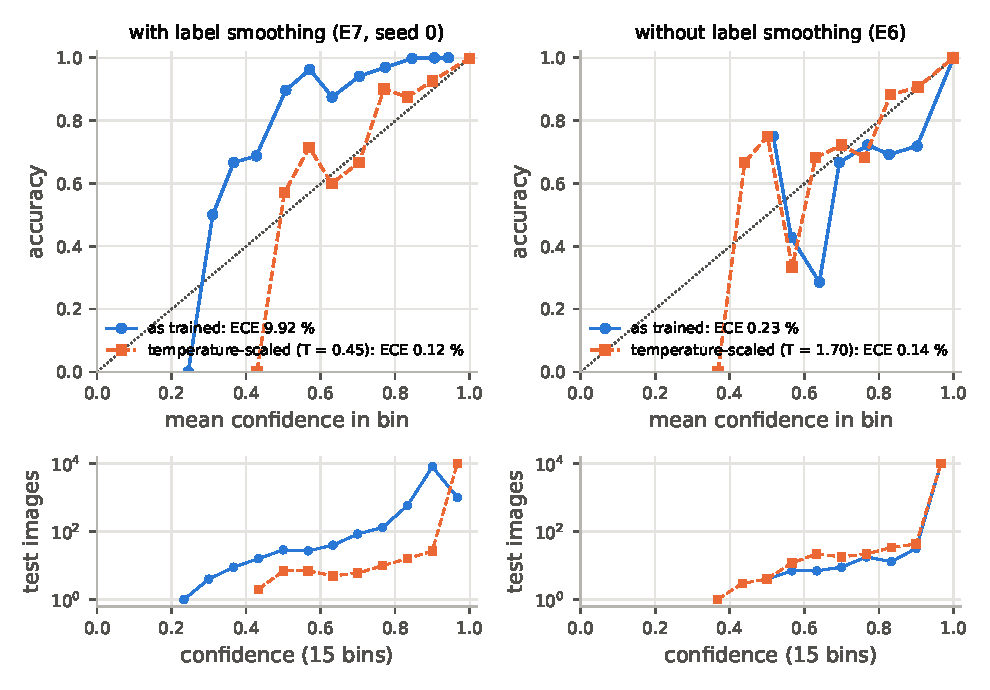
\includegraphics[width=0.68\textwidth]{figures/calibration.pdf}
  \caption{Reliability diagrams on the test set (top; dotted: perfect calibration) and the number
    of test images per confidence bin (bottom, log scale), as trained and after temperature
    scaling. Bins with few images are noisy. Left: with label smoothing almost all images sit in
    the bin around 0.9 while about 99.7\,\% of them are correct. Right: without label smoothing
    almost all images have a confidence close to 1.}
  \label{fig:calibration}
\end{figure}

With label smoothing the models are clearly under-confident (Table~\ref{tab:calibration},
Figure~\ref{fig:calibration}): the mean confidence of the final model is 89.8\,\% at
99.68\,\% accuracy, so the ECE is almost exactly the difference, 9.9 points. This is the same
effect as the loss floor in Section~\ref{sec:experiments}: the training target for the true
class is 0.91. Temperature scaling with $T \approx 0.45$ (it sharpens the distribution) removes
it: the ECE drops to about 0.1\,\% and the test cross-entropy by a factor of nine, consistently
over the three seeds. The model trained without label smoothing is instead slightly
over-confident ($T = 1.70$) with a small ECE of 0.23\,\%. After scaling both are equally well
calibrated, and the label-smoothed model keeps its 0.1 points higher accuracy. For a downstream
use that needs probabilities (thresholds, rejecting uncertain images), the final model should
therefore be used with $T = 0.45$.

\paragraph{The remaining errors.} Figure~\ref{fig:errors} (Appendix~\ref{app:tables}) shows all 32
misclassified test images of the final model with their top-3 probabilities. Most are genuinely hard (open loops,
heavy strokes, unusual slants); for some of them the given label itself is debatable. Whether
such images are label errors is the subject of Section~\ref{sec:curation}.

\section{Label curation}
\label{sec:curation}

\paragraph{Out-of-fold predictions.} To judge a label, the model must not have learnt it. The
60\,000 training images (training and validation split together) are divided into five
stratified folds of \num{12000} (fixed seed, committed list). Five models with the final
configuration (E7, 120 epochs, seed 0, deterministic) are trained, each on four folds, and
predict the fifth; every model keeps its last epoch, so the held-out fold does not even select
the checkpoint. This gives each training image a probability vector $p_i \in \R^{10}$ from a
model that never saw it. The test images get the mean of the five models' probabilities.

\paragraph{Confident learning.} Following Northcutt, Jiang and Chuang (2021), let $\tilde y_i$
be the given label of image $i$, $n_j$ the number of images labelled $j$ and $p_{ij}$ the
predicted probability of class $j$. The per-class threshold is the average self-confidence of
the class,
\[
  t_j = \frac{1}{n_j} \sum_{i : \tilde y_i = j} p_{ij}.
\]
Image $i$ is \emph{confidently} of class $j$ if $p_{ij} \ge t_j$; with several such classes the
most probable one counts, with none the image is not counted:
\[
  \hat y_i = \operatorname*{arg\,max}_{j : p_{ij} \ge t_j} p_{ij}.
\]
Per-class thresholds instead of a fixed level such as 0.5 make the rule robust against classes
the model is generally more or less confident about (with label smoothing every confidence is
about 0.9). The \emph{confident joint} counts the pairs of given and confident class,
$C_{kj} = |\{i : \tilde y_i = k,\ \hat y_i = j\}|$. Rescaling each row to the class size,
$\tilde C_{kj} = C_{kj} \, n_k / \sum_{j'} C_{kj'}$, and dividing by $n$ gives an estimate $Q$ of
the joint distribution of given and true label; $n\,(1 - \operatorname{tr} Q)$, the off-diagonal
mass of $\tilde C$, estimates the number of label errors. An image is \emph{flagged} if it lies off
the diagonal of $C$ ($\hat y_i$ exists and differs from $\tilde y_i$): the model is confidently
sure of another class. The flagged images are ranked by their self-confidence
$p_{i \tilde y_i}$, lowest first; this order is the review queue. (Northcutt et al.\ also prune
by the estimated noise rates; here the simple off-diagonal rule is used, and the estimate from
$\tilde C$ serves as a check of how many errors to expect.)

\paragraph{Results with the label-smoothed models.} The five fold models reach
$99.68 \pm 0.03\,\%$ test accuracy each, their ensemble 99.73\,\% (27 errors), and the
out-of-fold accuracy is 99.61\,\%. Confident learning, however, flags only 10 training images
and no test image. The reason is again label smoothing: every confidence is capped near 0.91,
so the thresholds $t_j$ lie between 0.901 and 0.910, right at the ceiling, and an image is
confidently of class $j$ only if the model is as sure of $j$ as it can be at all. Temperature
scaling moves the thresholds along with the confidences and raises the flags only to 38 and 5.
The review queue therefore also contains every image whose self-confidence is below 0.5
(the model gives the label less than even odds), ranked by self-confidence: 371 training and
47 test candidates, including every image whose prediction differs from its label. To see
whether confident learning works on a model without label smoothing, the folds are repeated
with $\varepsilon = 0$.

\paragraph{Without label smoothing.} The five fold models without label smoothing reach
$99.66 \pm 0.03\,\%$ test accuracy each and $99.71\,\%$ as an ensemble (29 errors); the
out-of-fold accuracy is 99.62\,\% (228 disagreements). The accuracy is the same as with label
smoothing, but the probabilities are not: the median self-confidence is 1.0 and the
out-of-fold predictions are over-confident ($T = 2.2$, ECE 0.26\,\%). The thresholds $t_j$ now
lie between 0.993 and 0.998 (test: 0.992--0.999), and confident learning works as intended:
it flags 61 training images, and the calibrated joint estimates 62 label errors; on the test
set it flags 2 and estimates 2 (Table~\ref{tab:cl}). With the same rule as above (flagged, or
self-confidence below 0.5) the review queue has 231 training and 30 test candidates: 61 flagged
plus 170 that are only uncertain, and 2 plus 28 on the test set; 200 of these 261 candidates
are also in the queue of the label-smoothed models. This queue was reviewed.

\begin{table}[t]
  \centering
  \small
  \caption{Confident learning on the out-of-fold predictions (training images) and the fold
    ensemble (test images), with and without label smoothing (LS). Estimate: off-diagonal mass
    of the calibrated joint $\tilde C$. Candidates: flagged or self-confidence below 0.5.}
  \label{tab:cl}
  \begin{tabular}{lrrrrrr}
    \toprule
    & \multicolumn{3}{c}{training images (60\,000)} & \multicolumn{3}{c}{test images (10\,000)} \\
    \cmidrule(lr){2-4} \cmidrule(lr){5-7}
    & thresholds $t_j$ & flagged / est. & cand. & thresholds $t_j$ & flagged / est. & cand. \\
    \midrule
    with LS & 0.902--0.909 & 10 / 13 & 371 & 0.901--0.910 & 0 / 0 & 47 \\
    without LS & 0.993--0.998 & 61 / 62 & 231 & 0.992--0.999 & 2 / 2 & 30 \\
    \bottomrule
  \end{tabular}
\end{table}

\paragraph{Review.} The decision rules were fixed in \texttt{curation/README.md} before the
first image: \emph{relabel} only if the true digit is unambiguous to a human, \emph{drop} if the
image is unreadable, not a digit or two digits, \emph{keep} if it is ambiguous but the label is
plausible, \emph{unsure} for a second look. All 261 candidates were reviewed in the workbench
in one round (median 6\,s per image, about 40 minutes of active work); the decisions are
\texttt{curation/decisions.csv}, dataset version \texttt{387ebdf5} (the E8 run folders record \texttt{efef0a05} for the same labels: the version then hashed the whole file, timestamps included). Table~\ref{tab:review}
gives the outcome, Figure~\ref{fig:curation} examples.

\begin{table}[t]
  \centering
  \small
  \caption{Curation round 1: decisions per split and for the candidates flagged by confident
    learning vs.\ those in the queue only for low self-confidence. Changed: relabel or drop.}
  \label{tab:review}
  \begin{tabular}{lrrrrr}
    \toprule
    Candidates & reviewed & keep & relabel & drop & changed \\
    \midrule
    training, flagged & 61 & 30 & 21 & 10 & 51\,\% \\
    training, low confidence only & 170 & 111 & 30 & 29 & 35\,\% \\
    training, all & 231 & 141 & 51 & 39 & 39\,\% \\
    test, flagged & 2 & 2 & 0 & 0 & 0\,\% \\
    test, low confidence only & 28 & 22 & 1 & 5 & 21\,\% \\
    \midrule
    total & 261 & 165 & 52 & 44 & 37\,\% \\
    \bottomrule
  \end{tabular}
\end{table}

\begin{figure}[t]
  \centering
  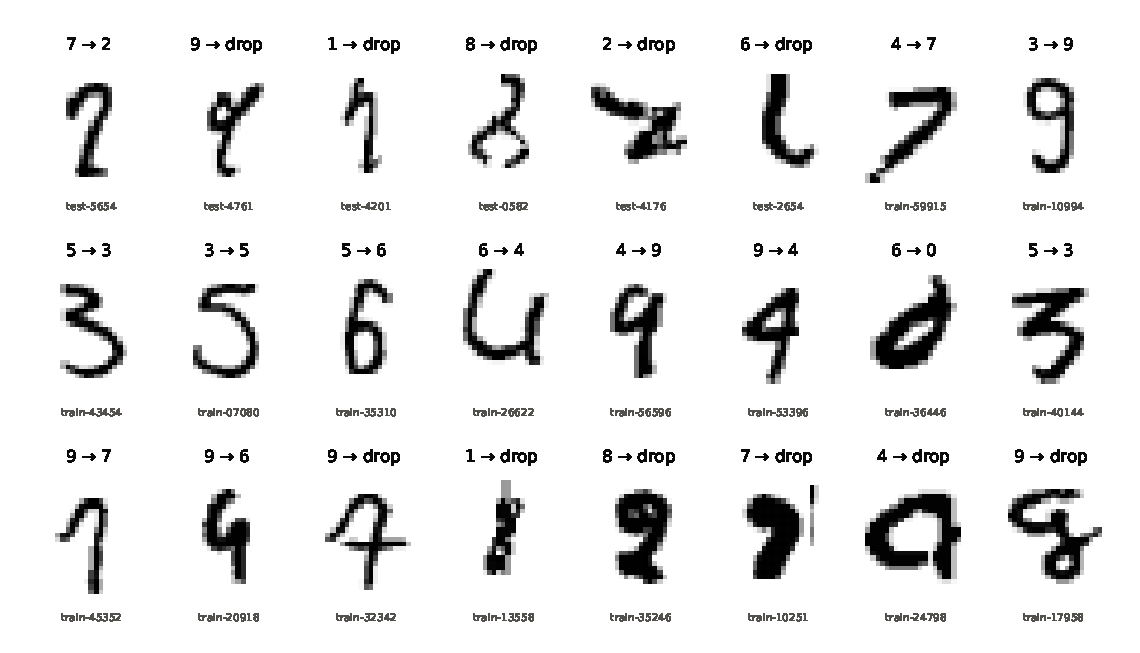
\includegraphics[width=0.72\textwidth]{figures/curation.pdf}
  \caption{Examples of curation decisions: all six changed test images (first row up to
    \texttt{test-2654}), then the first twelve relabelled and six dropped training images in
    queue order. Title: given label $\to$ new label, or \emph{drop}.}
  \label{fig:curation}
\end{figure}

Three observations. First, the ranking works: 15 of the 25 highest-ranked training candidates
were changed, but only 22 of the last 81; the confident-learning flag has a clearly higher hit
rate (51\,\%) than low confidence alone (35\,\%), yet the uncertain-only part still contributes
59 of the 90 training changes, so the extended queue of D22 was worth it. Second, on the test
set the strict rules find little: 1 relabel and 5 drops, against about 15 label errors reported
in the literature. Most test candidates are poorly written but plausible digits, which the rules
keep; the reported number depends as much on the rules as on the data. Third, confirmation
bias, as far as it can be measured: in 215 of the 217 keep or relabel decisions the model
disagreed with the given label, and the decision followed the model in only 44 of them (all
relabels to the predicted class; 8 relabels went to a third class). The queue shows the model's
opinion, but the reviewer kept the given label in three quarters of the cases (163 of 215) where
the model contradicted it.

\paragraph{Retraining on the curated data (E8).} The curation changes 90 of the 60\,000 training
images (0.15\,\%: 51 relabels, 39 drops; two relabels and six drops in the validation
split) and 6 of the
10\,000 test images. E8 repeats E7 exactly (same configuration, seeds and deterministic kernels)
on the curated training and validation data. Table~\ref{tab:curated} compares both on the
curated validation set, which is the same 5\,994 images for both, and on the original and the
curated test set (9\,995 images). The test predictions of a model are the same in both views;
only the labels and the five dropped images differ. The candidates were found with the fold
models, not with the E7 or E8 models (plan: use different models for finding and for
evaluation).

\begin{table}[t]
  \centering
  \small
  \caption{Original vs.\ curated data: accuracy in \%, mean $\pm$ standard deviation over seeds
    0--2, test errors per seed in brackets. Val: the curated validation split (5\,994 images) for
    both. Test original: all 10\,000 images with the original labels; test curated: without the
    five dropped images and with one label corrected.}
  \label{tab:curated}
  \begin{tabular}{llll}
    \toprule
    Training data & val (curated) & test original & test curated \\
    \midrule
    original (E7) & $99.83 \pm 0.02$ & $99.67 \pm 0.03$ (32, 31, 36) & $99.70 \pm 0.04$ (27, 29, 34) \\
    curated (E8) & $99.86 \pm 0.02$ & $99.60 \pm 0.09$ (49, 32, 39) & $99.62 \pm 0.07$ (46, 32, 35) \\
    \bottomrule
  \end{tabular}
\end{table}

Training on the curated data does not improve the model measurably. On the validation set E8 is
0.03 points better (about two images), on the original test set 0.07 points worse; both
differences are below the 0.15 points that are meaningful at this sample size
(Section~\ref{sec:calibration}), the test difference comes mostly from seed 0 of E8 (49 errors,
the other two 32 and 39), and a Welch test over the three seeds gives $p = 0.29$. Sixteen test
images are misclassified by all three E7 models and eighteen by all three E8 models, twelve of
them by both. 0.15\,\% wrong or unreadable labels are little noise for a regularised CNN
trained with label smoothing and augmentation. The curated test set changes the picture of the evaluation more than the
curated training set changes the model: of the six changed test images, the E7 models got five
(seed 0) or three (seeds 1 and 2) wrong, so 8--16\,\% of their errors are images whose label is
wrong or that cannot be read; on the curated test set the final model makes 27 instead of 32
errors. These numbers are an additional view, as the plan demands: the original test set stays
the reference, and no decision in this project was taken on the curated one.

\FloatBarrier
\section{Lessons learnt}
\label{sec:lessons}

\paragraph{A regulariser changes more than the accuracy.} Label smoothing was worth about 0.1
points of test accuracy, and it touched everything downstream: it put a floor under the
validation loss that broke early stopping (Appendix~\ref{app:earlystop}), it made the model
under-confident by ten points (Section~\ref{sec:calibration}), and it capped the probabilities
so that the confident-learning thresholds collapsed (Section~\ref{sec:curation}).

\paragraph{Loss and accuracy measure different things.} The validation loss rose while the
validation accuracy rose in the full-batch runs, the small CNN and Adam's long runs: the
direction of the weights decides the class, their norm the confidence. Selecting on the loss
would have cost accuracy; temperature scaling repairs the confidence afterwards.

\paragraph{Know the noise floor before reading a table.} With 10\,000 test images, differences
below about 0.15 points are noise; most of the sweep, the ablation and the E7/E8 comparison
lie inside it. Seeds and confidence intervals were cheap and prevented wrong conclusions.

\paragraph{Guarantees hold for the function they are stated for.} The Armijo line search
guarantees a decrease of the loss it evaluates; on a mini-batch that is not the training loss,
and the runs collapsed like plain SGD, while the full batch behaved exactly as predicted.

\paragraph{Curation cleans the evaluation more than the model.} At MNIST's label quality a
review round of 261 images changed 0.15\,\% of the training data and did not change the model
measurably, but it explained up to 16\,\% of the final model's test errors. The review worked
because of its order: models that had not seen the images, rules fixed before the first
decision, a ranked queue, and recorded agreement with the model. The same loop transfers to
industrial image inspection, where labels are made under time pressure and errors cost more.

\paragraph{Plain files make analysis easy.} One folder per run with a JSON-lines metric log and
Parquet predictions let the workbench, the report figures and ad-hoc questions read the same
files; deterministic kernels made every final run reproducible for 6\,\% more run time.

\clearpage
\appendix

\section{Initialisation and optimisers}
\label{app:optim}

\subsection{Initialisation}
With independent zero-mean weights, $\operatorname{Var}\bigl(z^{(l)}_i\bigr) = n_{l-1}
\operatorname{Var}\bigl(W^{(l)}\bigr) \, \mathbb{E}\bigl[(a^{(l-1)})^2\bigr]$. If $z^{(l-1)}$ is
symmetric around zero, the ReLU keeps half of its second moment,
$\mathbb{E}[(a^{(l-1)})^2] = \tfrac12 \operatorname{Var}(z^{(l-1)})$. The variance of the
pre-activations stays constant from layer to layer if
\begin{equation}
  \operatorname{Var}\bigl(W^{(l)}\bigr) = \frac{2}{n_{l-1}},
\end{equation}
which is He initialisation: $W^{(l)}_{ij} \sim \mathcal N(0, 2/n_{l-1})$, $b^{(l)} = 0$.

\subsection{Optimisers}
Both optimisers are implemented by hand (\texttt{optim.py}). With gradient $g_t$ at step $t$:
\begin{align}
  \text{SGD with momentum:} \quad & v_t = \mu v_{t-1} + g_t, \qquad
    w_t = w_{t-1} - \eta\, v_t, \\
  \text{Adam:} \quad & m_t = \beta_1 m_{t-1} + (1 - \beta_1) g_t, \qquad
    s_t = \beta_2 s_{t-1} + (1 - \beta_2) g_t^2, \\
  & w_t = w_{t-1} - \eta\, \frac{m_t / (1 - \beta_1^t)}{\sqrt{s_t / (1 - \beta_2^t)} + \epsilon}.
\end{align}
The momentum form is the one of PyTorch (no $(1-\mu)$ damping), so that the PyTorch MLP of
experiment E3 can use the same hyperparameters; in a steady state the effective step size is
$\eta / (1 - \mu)$. The bias corrections of Adam make the first step exactly
$\eta \operatorname{sign}(g_1)$ (up to $\epsilon$), which is one of the unit tests. A third optimiser, gradient descent with an Armijo
line search, follows in Appendix~\ref{app:linesearch}.

\section{Gradient descent with line search}
\label{app:linesearch}
\label{sec:linesearch}

\subsection{Theory}
Plain gradient descent $w_{t} = w_{t-1} - \eta g_t$ only decreases the loss $L$ if the step is
small enough: for an $L$-smooth function (gradient Lipschitz with constant $K$) every
$\eta < 2/K$ works, and a larger $\eta$ can make $L$ grow and the iteration diverge. The
classical remedy from optimisation courses is a backtracking line search with the Armijo
condition. Starting from $t = \eta$, the step is halved until it gives a sufficient decrease,
\begin{equation}
  L(w - t g) \le L(w) - c\, t\, \lVert g \rVert^2, \qquad t \in \{\eta, \beta\eta, \beta^2\eta,
  \dots\}, \quad c = 10^{-4}, \ \beta = \tfrac12,
  \label{eq:armijo}
\end{equation}
and $w - t g$ becomes the next iterate (\texttt{sgd\_ls}, without momentum). For an $L$-smooth
function the condition holds for every $t \le 2(1 - c)/K$, so the search stops after finitely
many halvings with $t \ge \min(\eta, \beta \cdot 2(1-c)/K)$. Summing the guaranteed decreases
gives $\sum_t \lVert g_t \rVert^2 < \infty$, hence $g_t \to 0$; for a convex $L$ with a unique
minimiser the iterates converge to it, whatever $\eta$ is.

We log the \emph{shortening factor} $\beta^k = t/\eta$ of every step, where $k$ is the number of
halvings. In the mini-batch version, $L$ and $g$ are the loss and gradient of the current
mini-batch, and the trial losses have to be evaluated with the same dropout masks and without
updating BatchNorm statistics, otherwise~\eqref{eq:armijo} compares two different functions. In
the full-batch version, $L$ is the mean loss over all \num{54000} training images, so the
guarantees above apply to the training loss itself.

\subsection{Experiment E2b}

\paragraph{E2b: SGD with line search on mini-batches.} SGD without momentum and with the
backtracking line search of Section~\ref{sec:linesearch}, start step $\eta = 1$, batch size 128,
in the NumPy network and in PyTorch (a unit test checks that both accept the same step sizes on
the same data; PyTorch runs it in float32, since the trial losses must not be rounded to
float16). After 20 epochs both are on the level of SGD with momentum (97.74\,\% test). The
line search hardly ever intervenes: the mean shortening factor is about 0.99 at the start and
still 0.96 in the ten epochs before the collapse. Over 500 epochs both runs collapse exactly like
plain SGD (epoch 126 and 134, validation accuracy 11.23\,\%), with a factor of 1 afterwards. The
Armijo condition only guarantees a decrease of the loss of the \emph{current} mini-batch; a step
that is good for 128 images can still increase the loss of the other \num{53872}, and that is
where the drift towards the dead second layer comes from. On mini-batches the line search
therefore does not provide the guarantee it is known for.

\paragraph{E2b: full-batch gradient descent with line search.} With \texttt{--full-batch}, every
step uses the gradient and the loss of the whole training set (PyTorch accumulates the gradient
over chunks of \num{2048} images, weighted by their share, which gives exactly the gradient of
the mean). This is the textbook setting of Section~\ref{sec:linesearch}, and it behaves like
the textbook (Figure~\ref{fig:fullbatch}). In all \num{20000} steps of both runs the training
loss decreases strictly; no step is rejected completely. The line search is active at the start:
in the first \num{1000} steps the accepted step is mostly $\tfrac14$ or $\tfrac18$ of $\eta = 1$
(mean factor 0.14--0.4). From about step \num{1000} on, the full step is accepted more and more
often, and after step \num{5000} it is always accepted, so the method turns into gradient descent
with $\eta = 1$. This fits the theory: the Hessian of the cross-entropy is proportional to
$p_y (1 - p_y)$, which shrinks as the network fits the training set, so the local smoothness
constant $K$ drops below 2 and the condition $t \le 2(1-c)/K$ holds for $t = 1$. There is no
collapse: the training accuracy reaches 100\,\% at step \num{1760} (PyTorch) and \num{2054}
(NumPy), and the training loss
falls to $2.5 \times 10^{-5}$ at step \num{20000}. Both implementations follow the same course;
PyTorch ends at 98.00\,\% test accuracy, which is better than SGD with momentum and close to
Adam, and the NumPy network at 97.94\,\%. The price is time: \num{20000} full-batch steps are
\num{20000} epochs (about 12 minutes on the GPU), against 20 epochs for the mini-batch
optimisers.

\begin{figure}[tb]
  \centering
  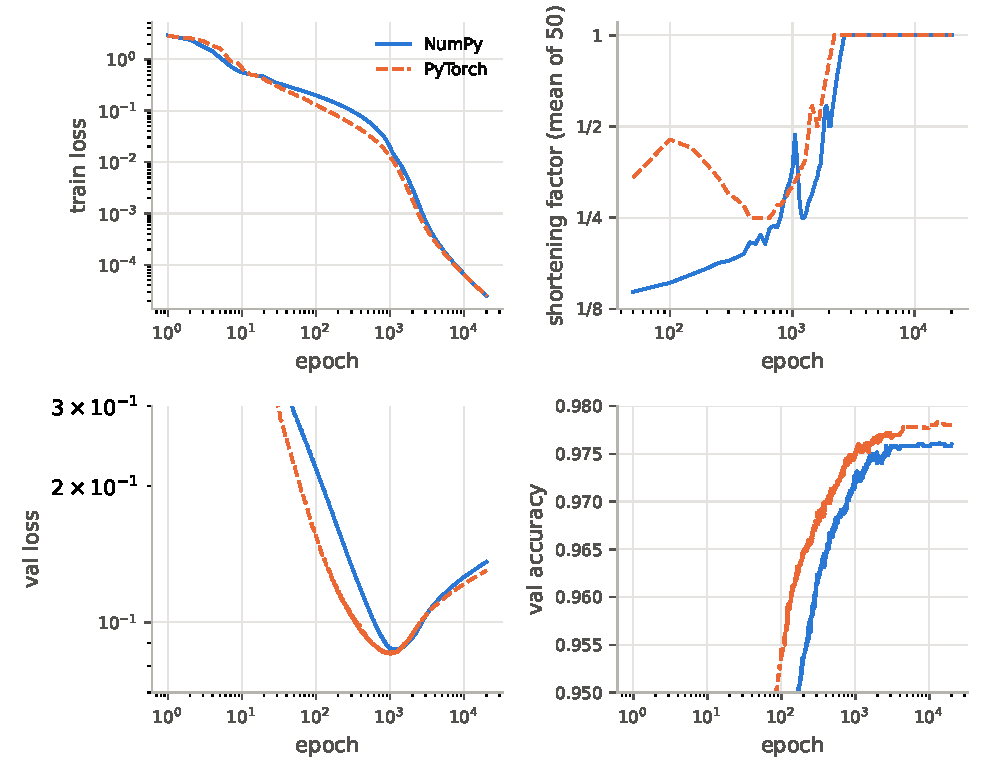
\includegraphics[width=0.9\linewidth]{figures/e2b_fullbatch.pdf}
  \caption{Full-batch gradient descent with line search, \num{20000} steps (one step per epoch,
    log scale). Top: training loss and the mean shortening factor $t/\eta$ over blocks of 50
    steps. Bottom: validation loss (log scale) and validation accuracy (zoomed). The validation
    loss is minimal at step 983 (PyTorch) and \num{1098} (NumPy) and then rises, while the
    validation accuracy keeps rising.}
  \label{fig:fullbatch}
\end{figure}

\subsection{Validation loss up, validation accuracy up}
\label{app:valloss}
 The full-batch runs show cleanly what
the mini-batch runs only hint at: after its minimum at step 983 (0.085, 97.50\,\%) the
validation loss of the PyTorch run rises by half, to 0.130 at step \num{20000}, while the
validation accuracy keeps rising to 97.83\,\% (step \num{12661}) and the test accuracy of that
checkpoint is the best of all MLP runs except Adam. To see how both can go up, we evaluated
four checkpoints of the run on the validation set and split the mean cross-entropy into the
part from correctly and from wrongly classified images (Table~\ref{tab:valloss}).

\begin{table}[tb]
  \centering
  \caption{Validation loss of the PyTorch full-batch run, split by correctness. Wrong: number of
    misclassified validation images; share: their part of the mean loss; mean: their mean loss;
    confidence: mean maximum softmax probability on the wrong images; $\lVert W^{(3)} \rVert_F$:
    norm of the output layer.}
  \label{tab:valloss}
  \begin{tabular}{rrrrrrrr}
    \toprule
    Step & Val loss & Val acc [\%] & Wrong & Share & Mean & Confidence &
      $\lVert W^{(3)} \rVert_F$ \\
    \midrule
    \num{1928}  & 0.094 & 97.68 & 139 & 0.085 & 3.66 & 0.81 & 7.6 \\
    \num{2000}  & 0.094 & 97.67 & 140 & 0.086 & 3.69 & 0.81 & 7.7 \\
    \num{12661} & 0.125 & 97.83 & 130 & 0.120 & 5.53 & 0.87 & 9.2 \\
    \num{20000} & 0.130 & 97.80 & 132 & 0.126 & 5.73 & 0.87 & 9.4 \\
    \bottomrule
  \end{tabular}
\end{table}

The 2.2\,\% misclassified images carry more than 90\,\% of the validation loss. Between step
\num{2000} and \num{12661}, 15 of them become correct and 5 correct ones become wrong, so the
accuracy rises by 10 images; but the remaining mistakes are made with more confidence (0.81
$\to$ 0.87 for the wrong class), and their mean loss rises from 3.7 to 5.5. The loss of the
correct images halves at the same time (0.008 $\to$ 0.005), but it is too small to matter. The
cause is the growth of the logits: once the training set is classified perfectly, the
cross-entropy can only decrease further by scaling up the margins, i.e.\ the weights, in
particular those of the output layer ($\lVert W^{(3)} \rVert_F$ 7.6 $\to$ 9.4; the standard
deviation of the validation logits grows from 8.7 to 14.6). The training loss goes to zero, but
there is no minimiser: gradient descent on separable data with the cross-entropy lets
$\lVert w \rVert$ grow without bound (slowly, logarithmically in the number of steps) while the
\emph{direction} of $w$ converges to a maximum-margin solution. This is proved for linear models
(Soudry et~al., 2018) and for homogeneous networks (Lyu and Li, 2020); the MLP with biases is
not homogeneous, but behaves the same way here. The
direction decides the predicted class and improves; the norm decides the confidence and
amplifies every remaining mistake. Accuracy and loss measure different things here, and
validation loss alone would have stopped training at step 983, 0.3 points below the best
accuracy. This is again a calibration problem (Section~\ref{sec:calibration}), and a simple
remedy is temperature scaling, which fixes the norm after training without changing the
predictions.

\section{Long runs and devices}
\label{app:long}

\begin{figure}[tb]
  \centering
  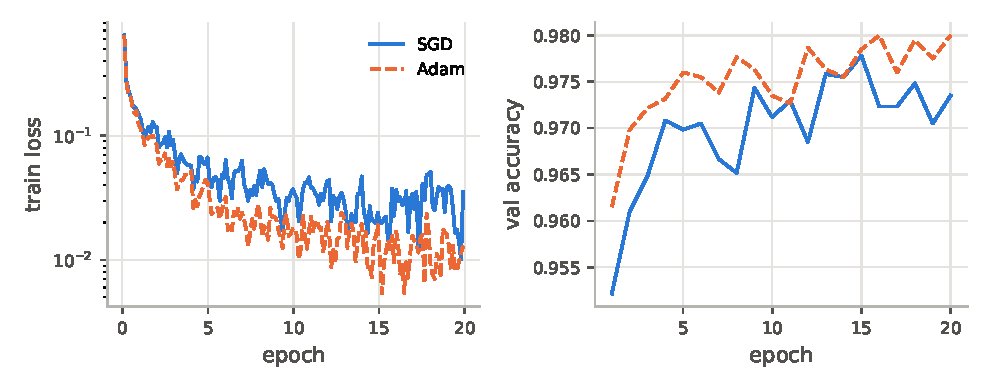
\includegraphics[width=\linewidth]{figures/e2_curves.pdf}
  \caption{E2, 20 epochs on the CPU. Left: training loss (mean over 50 steps, log scale);
    right: validation accuracy per epoch.}
  \label{fig:curves}
\end{figure}

\paragraph{Long runs: SGD collapses.} Trained for 300 epochs, SGD does not just stagnate, it
breaks down (Figure~\ref{fig:long}). For 100 epochs the training loss stays between 0.02 and
0.07 (median per epoch) and the validation accuracy between 96 and 98\,\%; from about epoch 105
the training loss rises to 0.5 and the validation accuracy sinks to 87\,\%, and in epoch 117 it
falls to 11.23\,\% and stays there. The run on the CPU, started for 900 epochs, collapsed in the same way in epoch 121 (it
was stopped after 337 epochs). In the last checkpoint all 128 units of the second hidden layer
are inactive for every validation image: the layer is dead, the logits are the constant
$b^{(3)}$, and the network predicts class~1 for every input. 11.23\,\% is exactly the share of
ones in the validation set, and the final training loss 2.303 equals the entropy 2.301 of the
class frequencies, which is the best a constant output can do. The collapse cannot heal itself:
by~\eqref{eq:relu} a dead layer passes $\delta^{(1)} = 0$ back, so $W^{(1)}$, $b^{(1)}$,
$W^{(2)}$, $b^{(2)}$ receive no gradient at all; only $b^{(3)}$ keeps moving, which is the
residual weight change of about 0.6 per 100 steps afterwards.

The weight-change metric shows the build-up: the $L_1$ distance of all weights to the weights 100
steps earlier grows from about $10^3$ to above $5 \times 10^3$ in the epochs before the collapse,
and the weight norms of the last checkpoint are three to eight times those of the best one
($\lVert W^{(l)} \rVert_F$ = 167, 253, 80 vs.\ 55, 36, 10). The likely mechanism is that, without
weight decay and with a constant effective step size of 1, the weights grow until one large
update pushes the pre-activations of the second layer below zero for all inputs. Because each
run keeps its best-validation checkpoint, the reported SGD numbers are not affected
(97.30\,\% test for the 300-epoch run). The fix belongs to the regularised models of the later
experiments: a learning-rate schedule, weight decay, and early stopping.

\begin{figure}[tb]
  \centering
  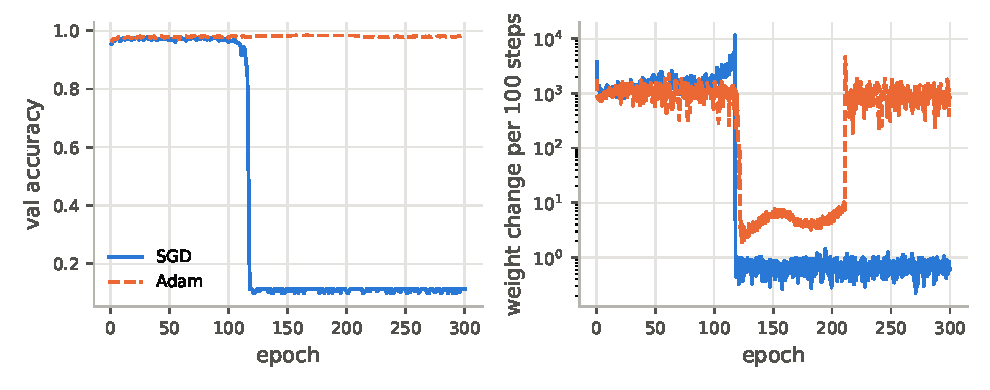
\includegraphics[width=\linewidth]{figures/e2_long.pdf}
  \caption{300 epochs on the GPU. Left: validation accuracy; right: weight change, the sum of
    $|w_t - w_{t-100}|$ over all parameters, logged every 100 steps (log scale).}
  \label{fig:long}
\end{figure}

\paragraph{Long runs: Adam memorises.} Adam does not collapse and gives the best result of the
series (98.44\,\% test). It fits the training set completely, though: the training loss falls
from about $5 \times 10^{-3}$ in epoch 100 to $10^{-8}$ in epoch 150 and below $10^{-10}$ in epoch
200, where the softmax probabilities of the true class round to 1 in float32 and many gradients
become exactly zero. The weight change drops by more than two orders of magnitude in this phase
(Figure~\ref{fig:long}, right). In epoch 212 the training loss jumps back to $10^{-2}$ and normal
training resumes. A plausible cause is Adam's normalisation: while the gradients are almost zero,
the second-moment estimate $s_t$ decays, and the next small but non-zero gradient is divided by
a tiny $\sqrt{s_t}$ and becomes a large step. Meanwhile the validation loss grows from 0.23
(epoch 120) to 0.45 (epoch 300) at an almost constant validation accuracy: the network becomes
overconfident in its mistakes. This is the starting point for the calibration analysis in
Section~\ref{sec:calibration}.

\paragraph{CPU and GPU.} With the same seed, both devices start from the same weights and see
the batches in the same order, and in float64 they agree to $10^{-10}$. In float32 the matrix
products on the GPU (cuBLAS) sum in a different order, and the tiny rounding differences grow
along the training trajectory: the 20-epoch runs end at 97.60 vs.\ 97.55\,\% (SGD) and 97.84
vs.\ 97.92\,\% (Adam), which is within the epoch-to-epoch noise. On the same device the runs
are deterministic: the 20- and 30-epoch SGD runs on the CPU select the same checkpoint (epoch
15) and give identical test results. The GPU does not pay off for this network: the median
throughput is \num{112000} vs.\ \num{71000} images/s for SGD and \num{74000} vs.\ \num{46000}
for Adam (CPU vs.\ GPU). With batches of 128 and only three matrix products per pass the GPU has
too little work per kernel, and reading the loss back to the host after every step synchronises
it each time.

\paragraph{GPU port.} The same code runs on the GPU with CuPy: the layers, the loss and the
optimisers take the array module of their arrays, \texttt{xp = numpy} or \texttt{xp = cupy}.
Initialisation and batch order come from the same NumPy random generator on both devices. In
float64, five SGD and Adam steps give the same weights on CPU and GPU up to a relative error of
$10^{-10}$ (\texttt{tests/test\_numpy\_net\_gpu.py}).

\section{Early stopping under label smoothing}
\label{app:earlystop}

\paragraph{Early stopping on a smoothed loss.} The first round of E5--E7 used 30 epochs and early
stopping on the validation loss with patience~5. Every one of the 18 runs was stopped, between
epoch 6 and 30, and most of them before the schedule had brought the learning rate down; one E7
run stopped after 6 epochs at 91\,\% of its maximum learning rate with the validation accuracy
still rising. The reason is label smoothing. With $\varepsilon = 0.1$ and $K = 10$ classes the
training target gives the true class probability $1 - \varepsilon + \varepsilon/K = 0.91$, so a
well-trained model is deliberately under-confident and its (unsmoothed) cross-entropy on a
correctly classified image cannot go much below $-\ln 0.91 \approx 0.094$. The validation loss
therefore reaches a floor near 0.1 after about 20 epochs and only wobbles by $\pm 0.01$ from
epoch to epoch, while the accuracy keeps improving (Figure~\ref{fig:earlystop}); patience~5
fires on this noise. The first round gave $99.61 \pm 0.12\,\%$ best validation and
$99.56 \pm 0.09\,\%$ test accuracy over the ten E5 runs, and the differences between the
settings mostly reflected when a run happened to stop. All runs below were therefore repeated
with 120 epochs and without early stopping; the checkpoint is still chosen by validation
accuracy. A run takes about 3.5 minutes.

\begin{figure}[t]
  \centering
  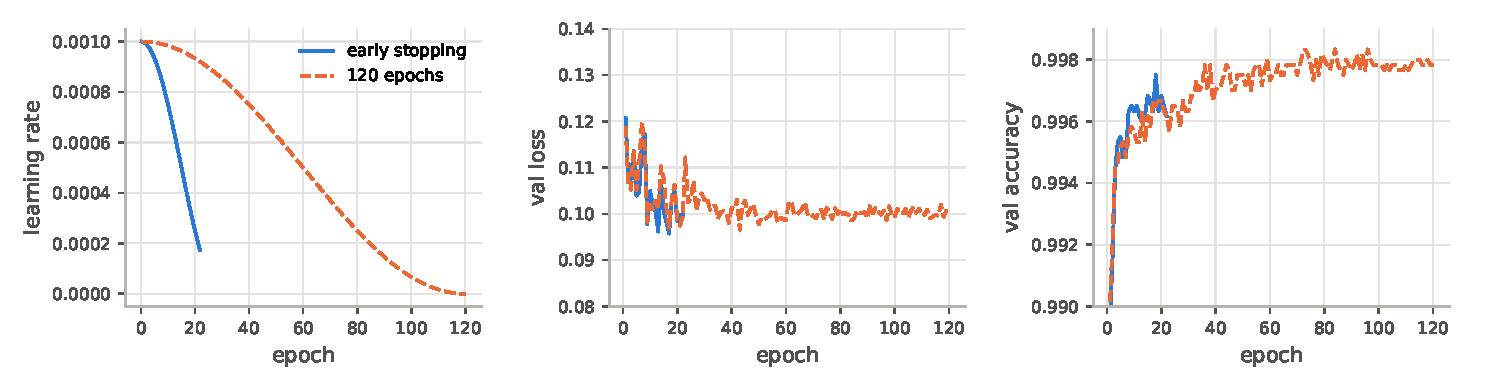
\includegraphics[width=\textwidth]{figures/e5_early_stop.pdf}
  \caption{E5 with learning rate $10^{-3}$ and cosine schedule: the first-round run (30-epoch
    schedule, stopped by early stopping after epoch 22) and the repeat with 120 epochs. After
    about 20 epochs the validation loss stays near the label-smoothing floor while the
    validation accuracy rises from 99.6 to 99.8\,\%.}
  \label{fig:earlystop}
\end{figure}

\FloatBarrier
\section{Full tables and the error gallery}
\label{app:tables}

Table~\ref{tab:results} lists every run of E1--E4 including the side experiments, Table~\ref{tab:perclass} and Figure~\ref{fig:confusion} the per-class metrics and the
confusion matrix of the final model, and Figure~\ref{fig:errors} all its test errors.

\begin{table}[tbp]
  \centering
  \small
  \setlength{\tabcolsep}{4pt}
  \caption{Results of E1--E4. Val: best validation accuracy (epoch); test: accuracy, macro-F1
    and mean cross-entropy of the selected checkpoint; time: wall-clock time of the whole run.
    For full-batch runs an epoch is a single step.}
  \label{tab:results}
  \begin{tabular}{llrrrrrr}
    \toprule
    Model & Device & Epochs & Val [\%] & Test [\%] & F1 [\%] & Test loss & Time [s] \\
    \midrule
    Logistic regression & CPU & -- & 91.98 & 92.54 & 92.43 & 0.276 & 5 \\
    $k$-NN ($k = 3$) & CPU & -- & 97.12 & 96.90 & 96.88 & 0.377 & 7 \\
    \midrule
    MLP, SGD & CPU & 20 & 97.78 (15) & 97.60 & 97.58 & 0.148 & 10 \\
    MLP, Adam & CPU & 20 & 98.00 (16) & 97.84 & 97.82 & 0.093 & 16 \\
    MLP, SGD & GPU & 20 & 97.58 (7) & 97.55 & 97.53 & 0.109 & 16 \\
    MLP, Adam & GPU & 20 & 97.97 (15) & 97.92 & 97.90 & 0.093 & 24 \\
    \midrule
    MLP, SGD & CPU & 30 & 97.78 (15) & 97.60 & 97.58 & 0.148 & 19 \\
    MLP, Adam & CPU & 30 & 98.18 (28) & 98.23 & 98.21 & 0.105 & 25 \\
    MLP, SGD & GPU & 300 & 97.78 (31) & 97.30 & 97.29 & 0.215 & 240 \\
    MLP, Adam & GPU & 300 & 98.42 (163) & 98.44 & 98.43 & 0.216 & 361 \\
    \midrule
    \multicolumn{8}{l}{\emph{E2b: SGD with line search ($\eta = 1$), NumPy}} \\
    mini-batch 128 & CPU & 20 & 97.75 (16) & 97.74 & 97.72 & 0.163 & 15 \\
    mini-batch 128 & CPU & 500 & 98.15 (29) & 97.92 & 97.89 & 0.190 & 446 \\
    full batch & GPU & 2\,000 & 97.52 (1\,959) & 97.73 & 97.72 & 0.083 & 88 \\
    full batch & GPU & 20\,000 & 97.62 (13\,585) & 97.94 & 97.93 & 0.117 & 652 \\
    \midrule
    \multicolumn{8}{l}{\emph{E3: PyTorch MLP; E2b with PyTorch}} \\
    MLP, SGD & GPU & 20 & 97.73 (17) & 97.60 & 97.59 & 0.166 & 13 \\
    MLP, Adam & GPU & 20 & 97.93 (19) & 97.90 & 97.88 & 0.106 & 15 \\
    MLP, SGD & GPU & 200 & 97.78 (39) & 97.76 & 97.74 & 0.259 & 128 \\
    MLP, Adam & GPU & 200 & 98.52 (108) & 98.40 & 98.39 & 0.169 & 140 \\
    MLP, line search, mini-batch & GPU & 20 & 97.82 (18) & 97.74 & 97.72 & 0.152 & 15 \\
    MLP, line search, mini-batch & GPU & 500 & 97.90 (81) & 97.77 & 97.76 & 0.396 & 478 \\
    MLP, line search, full batch & GPU & 2\,000 & 97.68 (1\,928) & 97.85 & 97.84 & 0.087 & 92 \\
    MLP, line search, full batch & GPU & 20\,000 & 97.83 (12\,661) & 98.00 & 97.99 & 0.118 & 712 \\
    \midrule
    \multicolumn{8}{l}{\emph{E4: small CNN, Adam}} \\
    CNN & GPU & 15 & 99.10 (13) & 98.95 & 98.94 & 0.046 & 18 \\
    CNN & GPU & 200 & 99.25 (194) & 99.12 & 99.12 & 0.105 & 205 \\
    \bottomrule
  \end{tabular}
\end{table}

\begin{table}[t]
  \centering
  \small
  \caption{Per-class precision and recall of the final model (E7, seed 0) on the test set.}
  \label{tab:perclass}
  \begin{tabular}{lrrrrrrrrrr}
    \toprule
    Digit & 0 & 1 & 2 & 3 & 4 & 5 & 6 & 7 & 8 & 9 \\
    \midrule
    Precision [\%] & 99.90 & 99.82 & 99.61 & 99.70 & 99.69 & 99.89 & 99.48 & 99.51 & 99.69 & 99.50 \\
    Recall [\%] & 100.00 & 99.56 & 99.90 & 99.90 & 99.29 & 99.55 & 99.69 & 99.51 & 99.79 & 99.60 \\
    \bottomrule
  \end{tabular}
\end{table}

\begin{figure}[t]
  \centering
  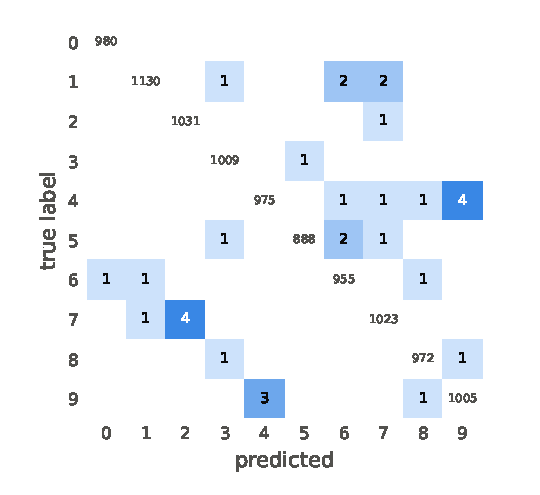
\includegraphics[width=0.48\textwidth]{figures/confusion.pdf}
  \caption{Confusion matrix of the final model on the test set (rows: true label). Off-diagonal
    counts are coloured; the diagonal shows the correct predictions as plain numbers.}
  \label{fig:confusion}
\end{figure}

\begin{figure}[t]
  \centering
  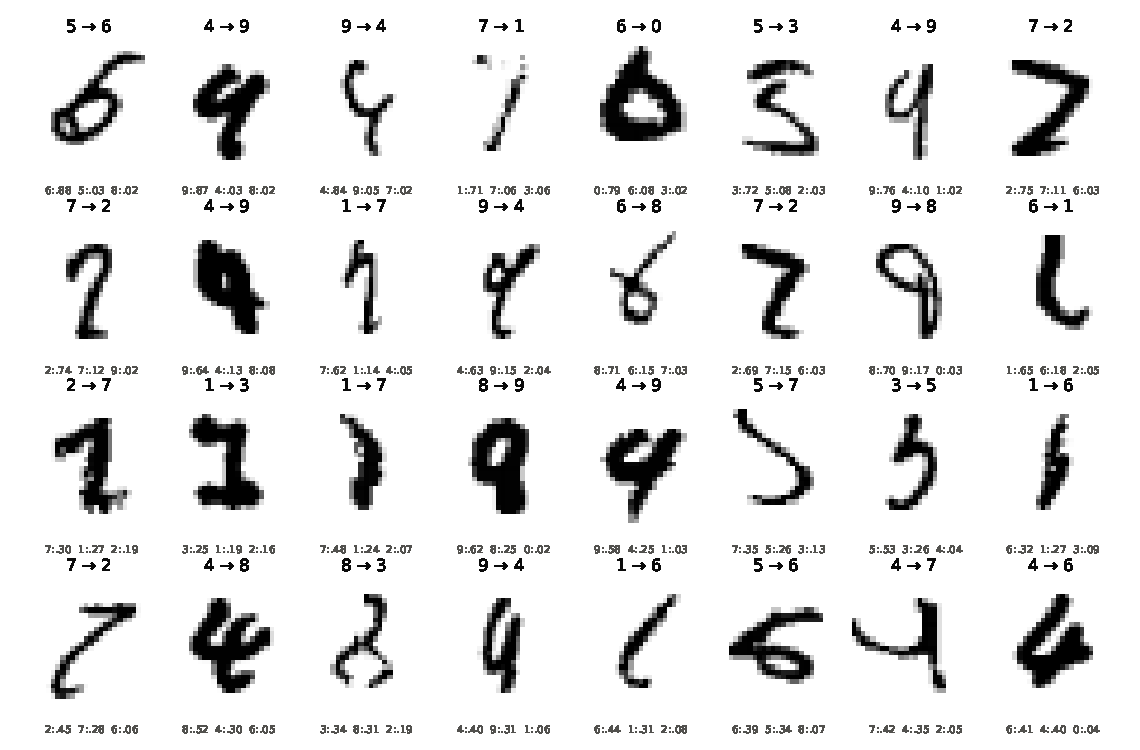
\includegraphics[width=\textwidth]{figures/errors.pdf}
  \caption{All 32 test errors of the final model, sorted by loss (highest first). Title: given
    label $\to$ prediction; below each image the top-3 classes with their probabilities (before
    temperature scaling).}
  \label{fig:errors}
\end{figure}

\end{document}
